%!TEX root = 1_a_Generalised IIT.tex
\section{Introduction}

\emph{Integrated Information Theory (IIT)}, developed by Giulio Tononi and collaborators, has emerged as one of the leading scientific theories of consciousness~\cite{oizumi2014phenomenology,marshall2016integrated,tononi2016integrated,mayner2018pyphi,koch2016neural}. At the heart of the theory is an algorithm which, based on the level of \emph{integration} of the internal functional relationships of a physical system in a given state, aims to determine both the quality and quantity (`$\Phi$ value') of its conscious experience.


While promising in itself, the mathematical formulation of the theory is not satisfying to date. The presentation in terms of examples and concomitant explanation veils the essential mathematical structure of the theory and impedes philosophical and scientific analysis. In addition, the current definition of the theory can only be applied to quite simple classical physical systems~\cite{Barrett.2014}, which is problematic if the theory is taken to be a fundamental theory of consciousness, and should eventually be reconciled with our present theories of physics.

To resolve these problems, we examine the essentials of the IIT algorithm and formally define a generalized notion of Integrated Information Theory.
This notion captures the inherent mathematical structure of IIT and offers a rigorous mathematical definition of the theory which has `classical' IIT 3.0 of Tononi et. al.~\cite{oizumi2014phenomenology, marshall2016integrated,mayner2018pyphi} as well as the more recently introduced \emph{Quantum Integrated Information Theory} of Zanardi, Tomka and Venuti~\cite{zanardi2018quantum} as special cases. In addition, this generalization allows us to extend classical IIT, freeing it from a number of simplifying assumptions identified in~\cite{BarrettMediano.2019}.

In the associated article~\cite{IITProcess} we show more generally how the main notions of IIT, including causation and integration, can be treated, and an IIT defined, starting from any suitable theory of physical systems and processes described in terms of category theory. Restricting to classical or quantum process then yields each of the above as special cases. This treatment makes IIT applicable to a large class of physical systems and helps overcome the current restrictions.

Our definition of IIT may serve as the starting point for further mathematical analysis of IIT, in particular if related to category theory~\cite{tsuchiya2016using,northoff2019mathematics}. It also provides a simplification and mathematical clarification of the IIT algorithm which 
extends the technical analysis of the theory \cite{Barrett.2014,tegmark2015consciousness,tegmark2016improved} and may
contribute to its ongoing critical discussion \cite{Bayne.2018,mediano2019measuring,mediano2019beyond,tononi2015consciousness}. The concise presentation of IIT in this article should also help to make IIT more easily accessible for mathematicians, physicists and other researchers with a strongly formal background.


\begin{figure}
\[
\scalebox{0.9}{
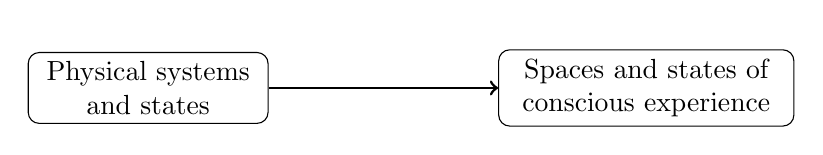
\begin{tikzpicture}[node distance = 18em, auto]
\tikzstyle{block} = [rectangle, draw, text centered, rounded corners]
\node [block, text width = 8em] (phys) {Physical systems and states};
% \node  [below=phys] {Physical state};
% \node [below=ment] {Experience};
\node [block, right of=phys, text width = 10em] (ment) {Spaces and states of \\conscious experience};
\draw [->, line width = 0.1em] (phys) edge (ment);
\node [style=label] at (6, .4) {$\Exp$};
\end{tikzpicture}
}
\]
\caption{\small An Integrated Information Theory specifies for every system in a particular state its conscious experience, described formally as an element of an experience space. In our formalization, this is a map
% \begin{equation}
\[ 
\! \! \! \! \! \! \! \! \! \! \! \! \! \! \! \! \!
\! \! \! \! \! \! \! \! \! \! \! \! \! \! \! \! \!
\! \! \! \! \! \! \! \! 
\Sys
\stackrel{\Exp}{\longrightarrow}  \Expcat 
\]
% \end{equation}
from the system class $\Sys$ into a class $\Expcat$ of experience spaces, which, first,
sends each system $S$ to its space of possible experiences $\Exp(S)$, and, second,
sends each state $s \in \St(S)$ to the actual experience the system is having when in that space,
\[
\! \! \! \! \! \! \! \! \! \! \! \! \! \! \! \! \!
\! \! \! \! \! \! \! \! \! \! \! \! \! \! \! \! \!
\St(S) \to \Exp(S) \qquad 
s \mapsto \Exp(S,s) \:.
\]
The definition of this map in terms of axiomatic descriptions of physical systems, experience spaces and further structure used in classical IIT is given in the first half of this paper.
}\label{FigureBox}
\end{figure}

\subsection{Structure of article}
We begin by introducing the necessary ingredients of a generalised Integrated Information Theory in Sections~\ref{sec:sys} to~\ref{sec:repertoires}, 
namely physical systems, spaces of conscious experience and cause-effect repertoires. Our approach is \emph{axiomatic} in that we state only the precise formal structure which is necessary to apply the IIT algorithm. In Section~\ref{sec:Integration}, we introduce a simple formal tool which allows us to present the definition of the algorithm of an IIT in a concise form in Sections~\ref{sec:alg-mech} and~\ref{sec:alg-sys}. Finally, in Section~\ref{sec:IITs}, we summarise the full definition of such a theory.

Following this we give several examples including IIT 3.0 in Section~\ref{sec:Classical} and Quantum IIT in Section~\ref{sec:quantum-IIT}. In Section~\ref{sec:problems} we discuss how our formulation allows one to extend classical IIT in several fundamental ways, before discussing further modifications to our approach and other future work in Section~\ref{sec:discussion}.  Finally, the appendix includes a detailed explanation of how our generalization of IIT coincides with its usual presentation in the case of classical IIT. 